Verify the Bonferroni inequality in (5--28) for $m = 3$.
\newline
\textit{Hint:} A Venn diagram for the three events $C_{1}$, $C_{2}$, and $C_{3}$ may help.
\newline
\par
Starting with 3 things:
\begin{enumerate}
    \item Denote:
    \begin{align*}
        C_{i}:          & True  & \text{ and } & P(C_{i}) = 1 - \alpha_{i}\\
        C_{i}^{\prime}: & False & \text{ and } & P(C_{i}^{\prime}) = 1 - P(C_{i}) = 1 - (1 - \alpha_{i}) = \alpha_{i}
    \end{align*}
    \item 
    \begin{align*}
        P(C_{1} \cap C_{2} \cap C_{3})
        +
        P({(C_{1} \cap C_{2} \cap C_{3})}^{\prime})
        &=
        1 \\
        P(C_{1} \cap C_{2} \cap C_{3})
        &=
        1
        -
        P({(C_{1} \cap C_{2} \cap C_{3})}^{\prime}) \\
        P(C_{1} \cap C_{2} \cap C_{3})
        &=
        1
        -
        P(C_{1}^{\prime} \cup C_{2}^{\prime} \cup C_{3}^{\prime})
    \end{align*}
    \item The Bonferroni inequality:
        \begin{align*}
            P(\bigcup_{i=1}^{3}{C_{i}}) \leq& \sum_{i=1}^{3}{P(C_{i})} \\
            \Rightarrow P(C_{1} \cup C_{2} \cup C_{3}) \leq& P(C_{1}) + P(C_{2}) + P(C_{3}) \\
            \Rightarrow P(C_{1}^{\prime} \cup C_{2}^{\prime} \cup C_{3}^{\prime}) \leq& P(C_{1}^{\prime}) + P(C_{2}^{\prime}) + P(C_{3}^{\prime}) \\
            \Rightarrow 1 - P(C_{1}^{\prime} \cup C_{2}^{\prime} \cup C_{3}^{\prime}) \geq& 1- \left[P(C_{1}^{\prime}) + P(C_{2}^{\prime}) + P(C_{3}^{\prime})\right] \\
        \end{align*}
\end{enumerate}

Using (5--28)
\begin{align*}
    P[\text{all }C_{i}\text{ true}] &= \\
    P(C_{1} \cap C_{3} \cap C_{3}) &= 1 - P[\text{at least one }C_{i}\text{ false}] & \text{(using 2.)} \\
    &= 1 - P(C_{1}^{\prime} \cup C_{2}^{\prime} \cup C_{3}^{\prime}) \\
    &\geq 1 - \left[P(C_{1}^{\prime}) + P(C_{2}^{\prime}) + P(C_{3}^{\prime})\right] & \text{(using 3.)} \\
    &= 1 - \left[(1 - P(C_{1})) + (1 - P(C_{2})) + (1 - P(C_{3}))\right] & \text{(using 1.)} \\
    &= 1 - \left(\alpha_{1} + \alpha_{2} + \alpha_{3}\right) & \text{(using 1.)}
\end{align*}

We could also draw some pictures instead. Creating a Venn diagram for the three events $\{C_{1}, C_{2}, C_{3}\}$. Each event only has two possibilities, True, or False, so we have $2^{3} = 8$ total possibilities. We could setup a square to represent these. To start we could partition the square into two columns the first (on the left) is True and the second is False to represent $C_{1}$.

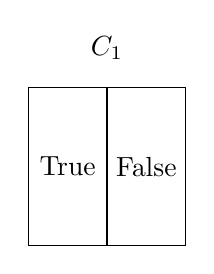
\begin{tikzpicture}
    % Draw the square
    \draw (0, 0) rectangle (2, 2);
    
    % Draw the vertical center line
    \draw (1, 0) -- (1, 2);
    
    \node at (1, 2.5) {$C_{1}$};
    \node at (0.5, 1) {True};
    \node at (1.5, 1) {False};

\end{tikzpicture}


Next, we could draw a horizontal line, so we have two rows to represent $C_{2}$. The first row is True and and second is False. This way we have all the combinations of events for $C_{1}$ and $C_{2}$ in the smaller boxes.

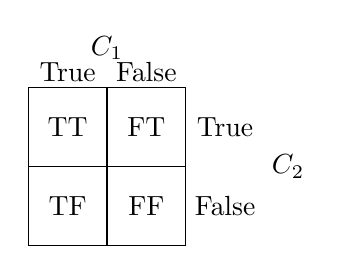
\begin{tikzpicture}
    % Draw the square
    \draw (0, 0) rectangle (2, 2);
    
    % Draw the vertical center line
    \draw (1, 0) -- (1, 2);
    
    \node at (1, 2.5) {$C_{1}$};
    \node at (0.5, 2.2) {True};
    \node at (1.5, 2.2) {False};

    % Draw the horizontal center line
    \draw (0, 1) -- (2, 1);

    \node at (2.5, 1.5) {True};
    \node at (2.5, 0.5) {False};
    \node at (3.3, 1) {$C_{2}$};
    
    \node at (0.5, 1.5) {TT};
    \node at (1.5, 1.5) {FT};
    \node at (0.5, 0.5) {TF};
    \node at (1.5, 0.5) {FF};

\end{tikzpicture}

Lastly, we can draw two horizontal lines that pass through the center to represent $C_{3}$. In each fo the smaller $C_{1}$ $C_{2}$ boxes the upper triangle is True and the lower triangle is False. We now have a visual representation of the sample space.

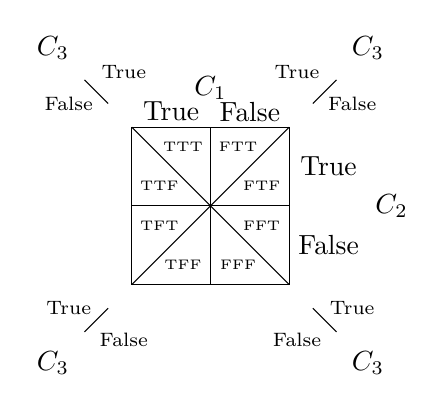
\begin{tikzpicture}
    % Draw the square
    \draw (0, 0) rectangle (2, 2);
    
    % Draw the vertical center line
    \draw (1, 0) -- (1, 2);
    
    \node at (1, 2.5) {$C_{1}$};
    \node at (0.5, 2.2) {True};
    \node at (1.5, 2.2) {False};

    % Draw the horizontal center line
    \draw (0, 1) -- (2, 1);

    \node at (2.5, 1.5) {True};
    \node at (2.5, 0.5) {False};
    \node at (3.3, 1) {$C_{2}$};
    
    \node at (0.65, 1.75) {\tiny{TTT}};
    \node at (0.35, 1.25) {\tiny{TTF}};

    \node at (1.35, 1.75) {\tiny{FTT}};
    \node at (1.65, 1.25) {\tiny{FTF}};

    \node at (0.35, 0.75) {\tiny{TFT}};
    \node at (0.65, 0.25) {\tiny{TFF}};

    \node at (1.65, 0.75) {\tiny{FFT}};
    \node at (1.35, 0.25) {\tiny{FFF}};

    % Draw the diagonal lines
    \draw (0, 0) -- (2, 2);
    \draw (0, 2) -- (2, 0);
    
    % Top-left C_3
    \node at (-1, 3) {$C_{3}$};
    \draw (-0.6, 2.6) -- (-0.3, 2.3);
    \node at (-0.1, 2.7) {\scriptsize{True}};
    \node at (-0.8, 2.3) {\scriptsize{False}};

    % Bottom-left C_3
    \node at (-1, -1) {$C_{3}$};
    \draw (-0.3, -0.3) -- (-0.6, -0.6);
    \node at (-0.1, -0.7) {\scriptsize{False}};
    \node at (-0.8, -0.3) {\scriptsize{True}};

    % Top-right C_3
    \node at (3, 3) {$C_{3}$};
    \draw (2.3, 2.3) -- (2.6, 2.6);
    \node at (2.1, 2.7) {\scriptsize{True}};
    \node at (2.8, 2.3) {\scriptsize{False}};

    % Bottom-right C_3
    \node at (3, -1) {$C_{3}$};
    \draw (2.3, -0.3) -- (2.6, -0.6);
    \node at (2.8, -0.3) {\scriptsize{True}};
    \node at (2.1, -0.7) {\scriptsize{False}};

\end{tikzpicture}
\newline
Here, everything's equal size, but that's not necessarily the case. Using (5--28)

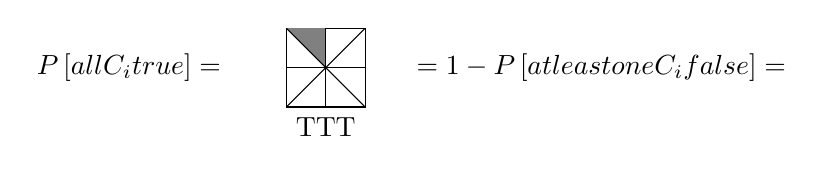
\begin{tikzpicture}[scale=0.5]

    \node at (-4, 1) {$P \left[ \text{all } C_{i}\text{ true} \right] = $};

    % Draw the square.
    \draw (0, 0) rectangle (2, 2);
    
    % Shade the TTT triangle.
    \fill[gray] (0, 2) -- (1, 2) -- (1, 1) -- cycle;

    % Draw the vertical center line.
    \draw (1, 0) -- (1, 2);
    
    % Draw the horizontal center line.
    \draw (0, 1) -- (2, 1);
    
    % Draw the diagonal lines.
    \draw (0, 0) -- (2, 2);
    \draw (0, 2) -- (2, 0);
    
    \node at (1, -0.5) {TTT};

    \node at (8, 1) {$=1
    -
    P \left[ \text{at least one } C_{i}\text{ false} \right] = $};

\end{tikzpicture}


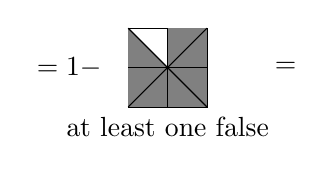
\begin{tikzpicture}[scale=0.5]

    \node at (-1.5, 1) {$ = 1- $};

    % Draw the square.
    \draw (0, 0) rectangle (2, 2);
    
    % Shade the top-right square.
    \fill[gray] (1, 1) -- (1, 2) -- (2, 2) -- (2, 1) -- cycle;

    % Shade the bottom square.
    \fill[gray] (0, 0) -- (0, 1) -- (2, 1) -- (2, 0) -- cycle;

    % Shade the TTF triangle.
    \fill[gray] (0, 1) -- (0, 2) -- (1, 1) -- cycle;

    % Draw the vertical center line
    \draw (1, 0) -- (1, 2);
    
    % Draw the horizontal center line
    \draw (0, 1) -- (2, 1);
    
    % Draw the diagonal lines
    \draw (0, 0) -- (2, 2);
    \draw (0, 2) -- (2, 0);
    
    \node at (1, -0.5) {at least one false};

    \node at (4, 1) {$ = $};

\end{tikzpicture}

\begin{tikzpicture}[scale=0.5]
    % Add "1-" in front of the first square
    \node at (-1.5, 1) {=1-};
    
    % Add left parenthesis before the squares
    \node at (-0.5, 1) {\Large $\bigg($};
    
    % Function to draw a square with a custom shaded triangle
    \newcommand{\drawSquareWithCustomShading}[4]{
        \draw (#1, 0) rectangle (#1+2, 2);
        \fill[#3] #2;
        \draw (#1+1, 0) -- (#1+1, 2);
        \draw (#1, 1) -- (#1+2, 1);
        \draw (#1, 0) -- (#1+2, 2);
        \draw (#1, 2) -- (#1+2, 0);
        \node at (#1+1, -0.5) {#4}; % Text below the square
    }
    
    % Draw the first square and shade TTF.
    \drawSquareWithCustomShading{0}{(0, 1) -- (0, 2) -- (0+1, 1) -- cycle}{gray}{TTF}
    
    % Add plus symbol after the first square
    \node at (2.5, 1) {$+$};
    
    % Draw the second square and shade TFT.
    \drawSquareWithCustomShading{3}{(3, 0) -- (3, 1) -- (3+1, 1) -- cycle}{gray}{TFT}
    
    % Add plus symbol after the second square
    \node at (5.5, 1) {$+$};
    
    % Draw the third square and shade TFF.
    \drawSquareWithCustomShading{6}{(6, 0) -- (6+1, 0) -- (6+1, 1) -- cycle}{gray}{TFF}
    
    % Add plus symbol after the third square
    \node at (8.5, 1) {$+$};
    
    % Draw the fourth square and shade FFF.
    \drawSquareWithCustomShading{9}{(9+1, 0) -- (9+2, 0) -- (9+1, 1) -- cycle}{gray}{FFF}
    
    % Add plus symbol after the fourth square
    \node at (11.5, 1) {$+$};
    
    % Draw the fifth square and shade FFT.
    \drawSquareWithCustomShading{12}{(12+2, 0) -- (12+2, 1) -- (12+1, 1) -- cycle}{gray}{FFT}
    
    % Add plus symbol after the fifth square
    \node at (14.5, 1) {$+$};
    
    % Draw the sixth square and shade FTF.
    \drawSquareWithCustomShading{15}{(15+1, 1) -- (15+2, 1) -- (15+2, 2) -- cycle}{gray}{FTF}
    
    % Add plus symbol after the sixth square
    \node at (17.5, 1) {$+$};
    
    % Draw the seventh square and shade FTT.
    \drawSquareWithCustomShading{18}{(18+1, 2) -- (18+2, 2) -- (18+1, 1) -- cycle}{gray}{FTT}

    % Add right parenthesis after the squares
    \node at (20.5, 1) {\Large $\bigg)$};

\end{tikzpicture}

\begin{tikzpicture}[scale=0.5] % Adjust the scale factor as needed

    \node at (-5, 1) {$\geq 1 - \mathlarger{\sum}_{i=1}^{3}{P \left( C_{i}\text{ false} \right)}= 1 - $};
    
    % Add left parenthesis before the squares
    \node at (-0.5, 1) {\Large $\bigg($};
    
    % Function to draw a square with a custom shaded triangle
    \newcommand{\drawSquareWithCustomShading}[4]{
        \draw (#1, 0) rectangle (#1+2, 2);
        \fill[#3] #2;
        \draw (#1+1, 0) -- (#1+1, 2);
        \draw (#1, 1) -- (#1+2, 1);
        \draw (#1, 0) -- (#1+2, 2);
        \draw (#1, 2) -- (#1+2, 0);
        \node at (#1+1, -0.5) {#4}; % Text below the square
    }
    
    % Draw C_{1} and shade false values.
    \drawSquareWithCustomShading{0}{(1, 0) -- (2, 0) -- (2, 2) -- (1, 2) -- cycle}{gray}{\scriptsize$C_{1} \text{False}$}
    
    % Add plus symbol after the first square
    \node at (2.5, 1) {$+$};
    
    % Draw C_{2} and shade false values.
    \drawSquareWithCustomShading{3}{(3+0, 0) -- (3+2, 0) -- (3+2, 1) -- (3+0, 1) -- cycle}{gray}{\scriptsize$C_{2} \text{False}$}
    
    % Add plus symbol after the second square
    \node at (5.5, 1) {$+$};
    
    % Draw C_{3} and shade false values.
    \fill[gray] (6+0, 1) -- (6+0, 2) -- (6+1, 1) -- cycle;
    \fill[gray] (6+0, 0) -- (6+1, 0) -- (6+1, 1) -- cycle;
    \fill[gray] (6+1, 0) -- (6+2, 0) -- (6+1, 1) -- cycle;
    \drawSquareWithCustomShading{6}{(6+1, 1) -- (6+2, 1) -- (6+2, 2) -- cycle}{gray}{\scriptsize$C_{3} \text{False}$}


    % Add right parenthesis after the squares
    \node at (9, 1) {\Large $\bigg) = $};

\end{tikzpicture}

\[
    =
    1
    -
    \mathlarger{\sum}_{i=1}^{3}{\left(1 - P \left( C_{i}\text{ true} \right)\right)}= 
\]

\begin{tikzpicture}[scale=0.5] % Adjust the scale factor as needed
    % Add "1 - (" in front of the first square
    \node at (-1.5, 1) {$ = 1 - \Biggl{(}$};
    
    % Function to draw a square with a custom shaded triangle
    \newcommand{\drawSquareWithCustomShading}[4]{
        \draw (#1, 0) rectangle (#1+2, 2);
        \fill[#3] #2;
        \draw (#1+1, 0) -- (#1+1, 2);
        \draw (#1, 1) -- (#1+2, 1);
        \draw (#1, 0) -- (#1+2, 2);
        \draw (#1, 2) -- (#1+2, 0);
        \node at (#1+1, -0.5) {#4}; % Text below the square
    }

    \node at (0.5, 1) {$\Biggl{(}$ $1 - $};
    
    % Draw C_{1} and shade true values.
    \drawSquareWithCustomShading{1.5}{(1.5+0, 0) -- (1.5+1, 0) -- (1.5+1, 2) -- (1.5+0, 2) -- cycle}{gray}{\scriptsize$C_{1} \text{True}$}
    
    % Add ") + (1-"
    \node at (5.0, 1) {$\Biggl{)} + \Biggl{(} 1- $};
    
    % Draw C_{2} and shade true values.
    \drawSquareWithCustomShading{6.5}{(6.5+0, 1) -- (6.5+2, 1) -- (6.5+2, 2) -- (6.5+0, 2) -- cycle}{gray}{\scriptsize$C_{2} \text{True}$}
    
    % Add ") + (1-"
    \node at (10.0, 1) {$\Biggl{)} + \Biggl{(} 1- $};
    
    % Draw C_{3} and shade true values.
    \fill[gray] (11.5+0, 0) -- (11.5+0, 1) -- (11.5+1, 1) -- cycle;
    \fill[gray] (11.5+0, 2) -- (11.5+1, 2) -- (11.5+1, 1) -- cycle;
    \fill[gray] (11.5+1, 2) -- (11.5+2, 2) -- (11.5+1, 1) -- cycle;
    \drawSquareWithCustomShading{11.5}{(11.5+1, 1) -- (11.5+2, 1) -- (11.5+2, 0) -- cycle}{gray}{\scriptsize$C_{3} \text{True}$}

    % Add "))"
    \node at (14.5, 1) {$\Biggl{)} \Biggl{)} =$};

\end{tikzpicture}
\[
    =
    1
    -
    \left(
        \alpha_{1}
        +
        \alpha_{2}
        +
        \alpha_{3}
    \right)
\]